% !TEX encoding = UTF-8
% !TEX TS-program = pdflatex
% !TEX root = ../tesi.tex
% !TEX spellcheck = it-IT

%**************************************************************
\chapter{Il progetto all'interno dell'azienda}
\label{cap:progetto-azienda}
%**************************************************************

\section{Presentazione del progetto}

Il progetto svolto da me durante l'attività di stage consiste nello sviluppo di un'applicazione mobile, sviluppata nativamente in Android, che replica il meccanismo e il flusso utente già esistente nel web integrandolo all'interno di questo tipo di piattaforma. 

\subsection{Motivazioni}

Come già presentato nel capitolo 1, CoffeeStrap ha come primo e unico scopo lo sviluppo di una piattaforma peer-to-peer per l'apprendimento di una lingua tramite interazioni tra utenti. Lo scopo principale in questa prima fase di sviluppo è quella di raccogliere un bacino utenti considerevole, in modo da poter capire su quale linea portare avanti l'idea e modellare quest'ultima in base al \textit{feedback} e al tipo di iterazione dell'utente medio. Prima dell'inizio del mio stage CoffeeStrap disponeva solamente dell'applicazione web, la quale possedeva circa 2000 iscritti e mediamente 15 utenti attivi al giorno. 

Il progetto di stage che ho svolto nasce dunque dalla necessità di affiancare all'applicazione web l'applicazione mobile, in modo da poter fornire all'utente più possibilità di utilizzo del prodotto ed arrivare inoltre ad un considerevole incremento del bacino utenti. La considerazione principale a monte di ciò è il fatto che oggigiorno l'utente medio spende la maggior parte del proprio tempo sul proprio smartphone piuttosto che sul proprio PC, per tutti i vantaggi legati alla tecnologia mobile. È di fatto una necessità imprescindibile per una start-up in ambito \textit{web/mobile} estendersi su più piattaforme se si vuole competere in un certo tipo di mercato ed ottenere dei finanziamenti. In aggiunta CoffeeStrap può essere categorizzato di fatto come \textit{social network}, ulteriore motivo per il quale sviluppare il prodotto su mobile è di importanza fondamentale.

L'avere a disposizione l'applicazione a qualsiasi ora del giorno e in qualsiasi luogo permette all'utente di fruire del prodotto senza limitazioni e nel momento esatto in cui ne sente la necessità. Da questo ne deriva un aumento del numero di iterazioni e della quantità di utenti attivi giornalieri, dati di fondamentale importanza per gli investitori.

Possiamo sintetizzare in cinque punti i vantaggi per cui un'azienda dovrebbe avere un'applicazione mobile:

\begin{enumerate}

\item \textbf{Visibilità}: i dati rilevati indicano che le ricerche all'interno degli \textit{App stores} siano molto elevate, motivo per cui comparire tra i risultati di ricerca rappresenta un'ottima \textbf{pubblicità} per l'azienda;
\item \textbf{Aumento del valore del brand}: avere la propria applicazione è indice di un'azienda \textit{dinamica}, sempre attenta all'evoluzione tecnologica e al passo coi tempi. Questi valori aumentano di molto il valore dell'azienda;
\item \textbf{Copertura mediatica}: con la tecnologia mobile è possibile coprire anche zone con scarsa connettività ad internet, coprendo una zona molto maggiore ed aprendo nuove possibilità per il business;
\item \textbf{Crescita del mercato mobile}: il mondo mobile è in grossa crescita e prospera più velocemente rispetto al web. Lo smartphone è al giorno d'oggi uno strumento essenziale per qualsiasi persona, sia per il tempo libero che per il lavoro.
\item \textbf{Capacità di differenziarsi dai concorrenti}: le aziende concorrenti che non dispongono di un'applicazione mobile passano in secondo piano rispetto ad un'azienda che ne dispone.

\end{enumerate}

\begin{figure}[htpd]
\centering
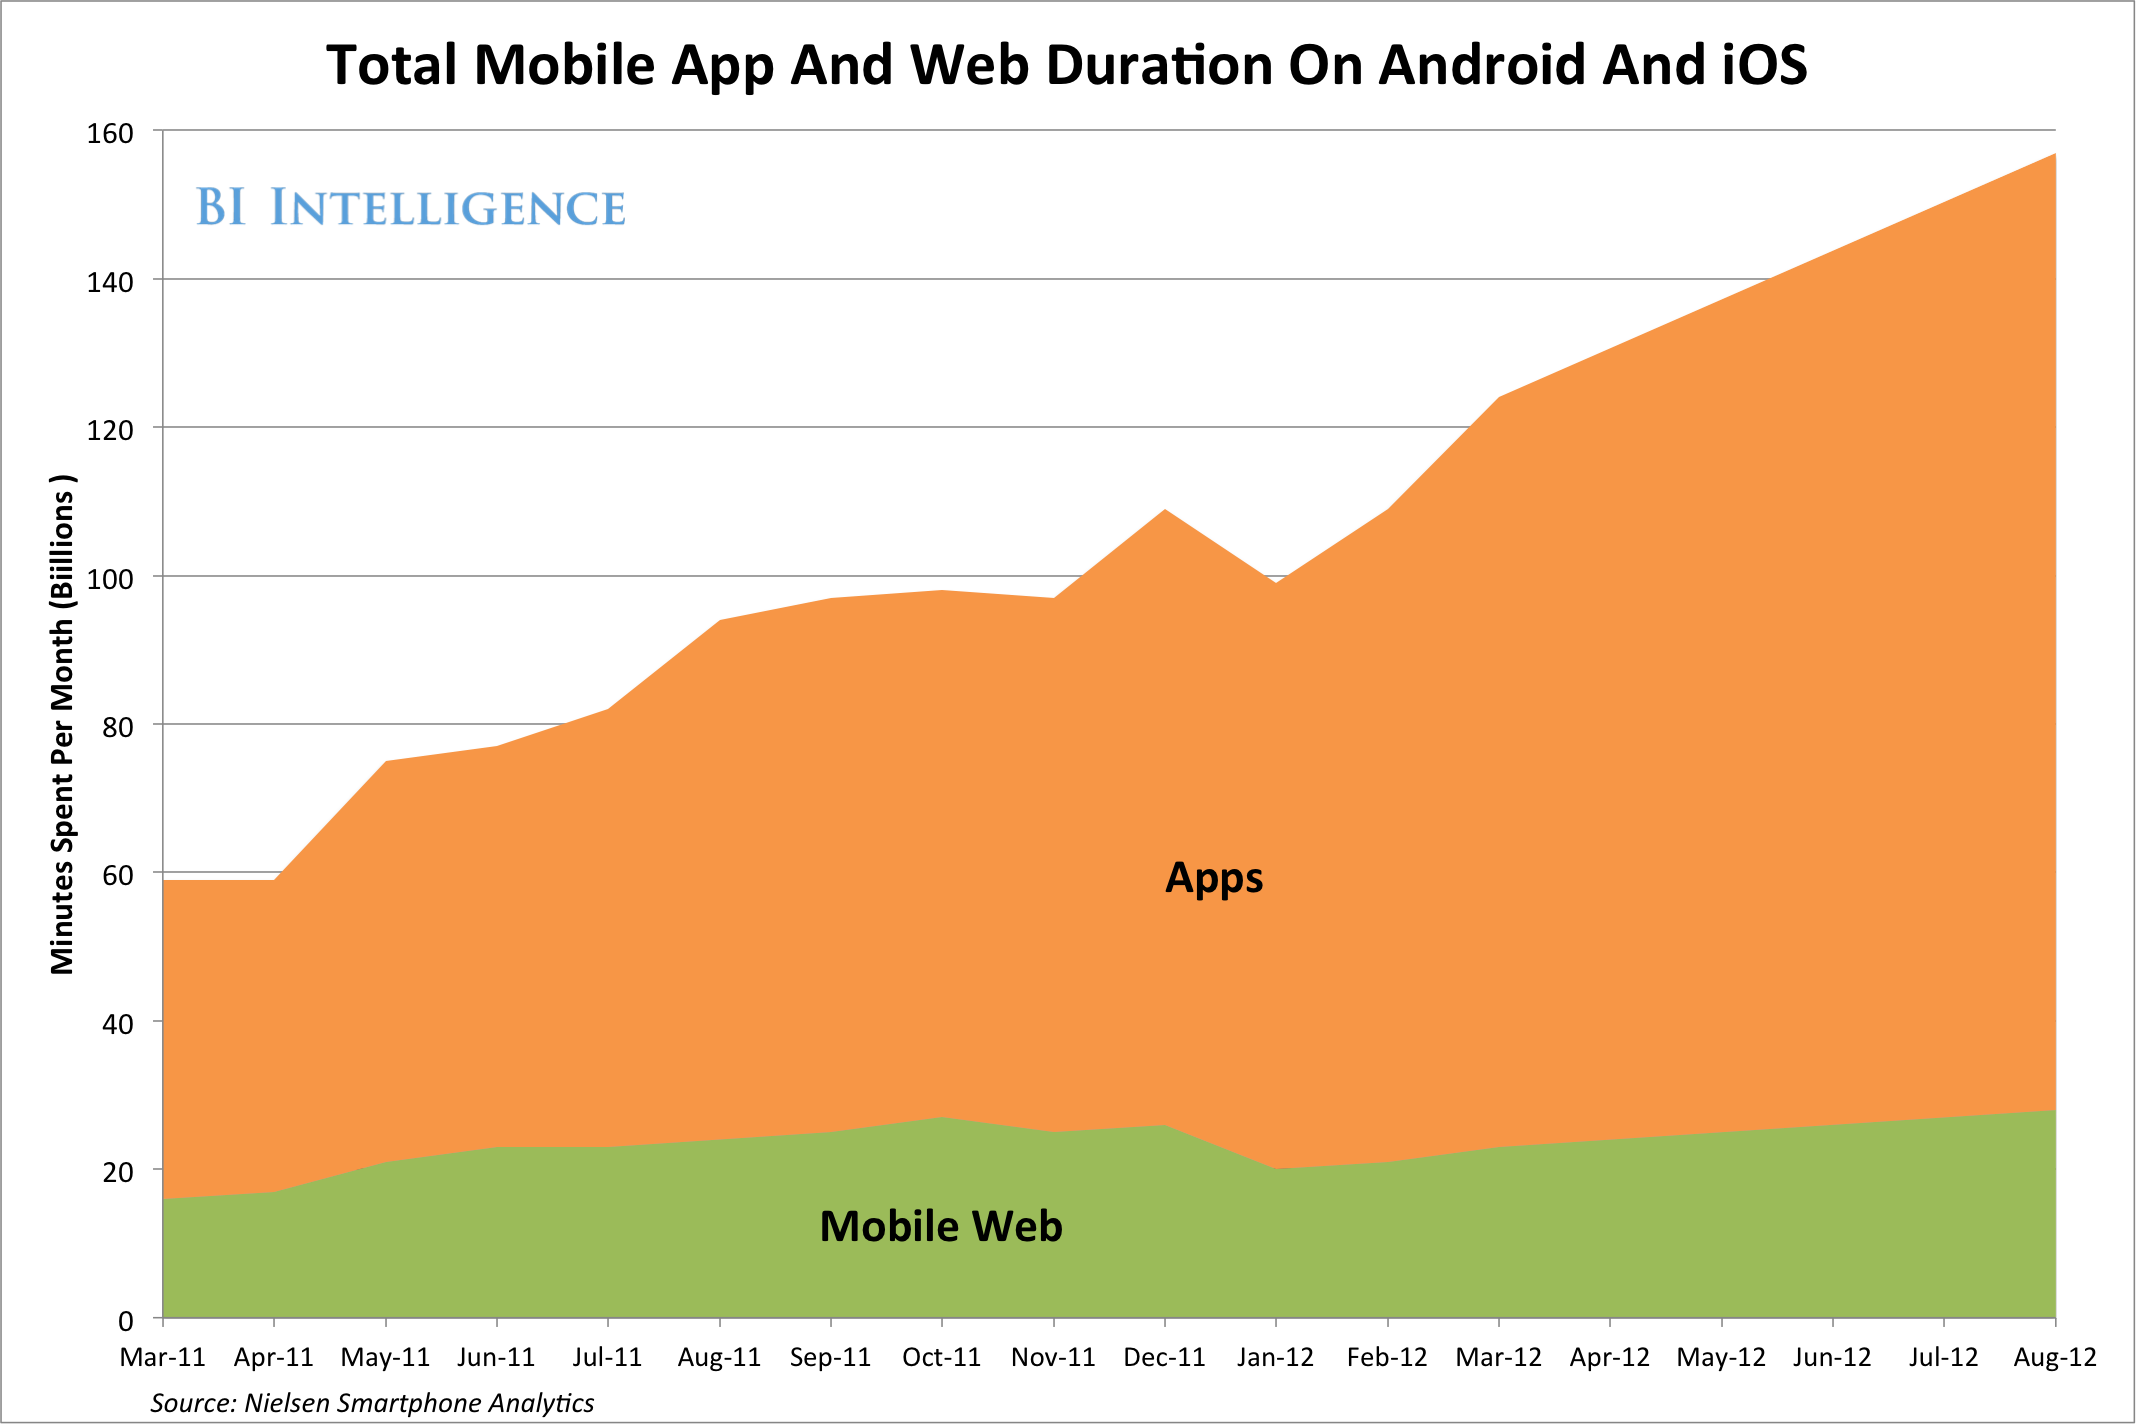
\includegraphics[width=\textwidth]{../immagini/mobile-and-web-market}
\caption{Comparazione di traffico web mobile e mobile app tra il 2011 e il 2012}  
\end{figure}

\subsection{Aspettative}

La mia preparazione e formazione in ambito di sviluppo mobile poteva ritenersi pari a zero all'inizio dell'attività di stage. Ciononostante l'azienda era consapevole di quali fossero le mie capacità, avendo già collaborato con me e il mio \textit{team} per il progetto di ingegneria del software dell'anno accademico 2013/2014. Pochi mesi prima, in collaborazione con il team \textbf{steakholders}, avevo infatti sviluppato un framework per l'amministrazione di dati provenienti da MongoDB. CoffeeStrap ha assunto il ruolo di \textbf{committente} all'interno di questo progetto, quindi vi erano state diverse interazioni tra me e l'azienda, la quale tuttora utilizza quotidianamente come strumento di supporto. Il progetto in questione si chiama \textbf{MaaP}, rilasciato sotto licenza MIT, disponibile come pacchetto all'interno di npm\footnote{\url{https://www.npmjs.com/package/maap}}. Inoltre su github\footnote{\url{https://github.com/steakholders/maap}} è disponibile il codice sorgente.

A fronte della realizzazione di questo progetto l'azienda poneva in me delle buone aspettative circa le tempistiche di apprendimento della tecnologia e di integrazione all'interno del team, per cui il \textbf{rischio} di ospitare un'attività di stage era mitigato da questi fattori. Inoltre i membri di CoffeeStrap, avendo frequentato anch'essi il mio stesso corso di studi, erano al corrente di quale tipo di formazione l'università di Padova offrisse agli studenti e in particolare in che modo e secondo quali prassi il corso di \textit{Ingegneria del Software} preparasse questi ultimi ad essere inseriti velocemente nel mondo del lavoro, avendo alle spalle un'esperienza corposa ed istruttiva. Queste motivazioni hanno fatto sì che l'azienda decidesse di ospitare al loro interno un'attività di stage che potesse soddisfare gli obiettivi preposti. 

Considerando la durata dello stage e le tempistiche legate all'apprendimento della tecnologia, l'aspettativa da parte dell'azienda era quella di arrivare alla fine del periodo di stage con in mano un \textbf{prototipo funzionante}, pronto per essere inserito in una fase successiva di test più approfondito e di raffinamento dei componenti, comunque non ancora sufficientemente maturo per essere inserito pubblicamente nel mercato. L'aspettativa era quella di una versione dell'applicazione che in ambito informatico viene generalmente indicata come \textit{beta}.

Gli obiettivi minimi delineati sono i seguenti:

\begin{itemize}

\item \textit{Signup} e \textit{login} all'applicazione da parte dell'utente;
\item Visualizzazione e modifica delle preferenze da parte dell'utente;
\item Comunicazione audio;
\item Sistema di notifica, quest'ultimo punto fondamentale all'interno del progetto;

\end{itemize}

Oltre agli obiettivi minimi inoltre sono stati posti degli obiettivi massimi:

\begin{itemize}

\item Comunicazione testuale;
\item Comunicazione video;

\end{itemize}

Durante il corso dell'attività di stage ciononostante i requisiti sono aumentati, in base alla necessità di realizzare appieno il flusso previsto, il quale è stato riprogettato nel medesimo periodo. Gli obiettivi sono dunque rimasti invariati ma sono stati aggiunti i seguenti:

\begin{itemize}

\item Richiesta di un \textbf{match} in base a una lingua, dove per \textit{match} si intende un \textit{collegamento} tra due utenti mantenibile nel tempo;
\item Notifica di invito da parte di un utente di parlare una lingua;
\item Creazione e mantenimento della lista di match;

\end{itemize}

Questi ultimi sono stati necessari per arrivare ad un'applicazione con un grado di usabilità accettabile.

\subsection{Obiettivi di formazione}

L'azienda, essendo di piccole dimensioni e in fase primordiale, ha come prima necessità, oltre allo sviluppo e diffusione del prodotto, la formazione di un team qualificato con all'interno elementi di natura tecnica.  Nelle aziende di questo tipo la prima necessità e risorsa sono le \textbf{persone}, in quanto il valore dell'azienda deriva dal lavoro dei suoi dipendenti. A fronte di questa necessità ospitare un'attività di stage permette all'azienda di poter integrare personale giovane, con una buona formazione e dotati di forte motivazione e stimoli, oltre che una buona elasticità mentale. 

Tra gli obiettivi formativi si delineano i seguenti:

\begin{itemize}

\item Apprendimento della tecnologia mobile, in particolare introduzione all'utilizzo della piattaforma Android;
\item Apprendimento del protocollo REST e comunicazione lato server tramite API;
\item Formazione sullo sviluppo di servizi di terze parti utilizzate dall'azienda; 
\item Introduzione alla metodologia agile scrum;
\item Introduzione al contesto della start-up e alla sua particolare realtà.
\item Comprensione dei limiti e delle potenzialità delle tecnologie utilizzate.

\end{itemize}

\section{Vincoli}

\subsection{Vincoli tecnologici}

All'inizio dello stage è stata fatta una valutazione riguardo lo \textit{stack tecnologico} da adottare per la realizzazione dell'applicazione. Sono state delineate tre possibilità:

\begin{itemize}

\item \textbf{Titanium}\footnote{\url{http://www.appcelerator.com/titanium/}}, un framework di sviluppo mobile basato su \textit{javascript} e \textit{HTML5}, che permette lo sviluppo su più piattaforme;

\item \textbf{Ionic}\footnote{\url{http://ionicframework.com/}}, altro framework ibrido molto simile al precedente;

\item \textbf{Nativo Android}, in cui viene messo a disposizione un vero e proprio SDK ufficiale\footnote{\url{http://developer.android.com/sdk/index.html}} per lo sviluppo, basato su Java.

\end{itemize}

Il vantaggio delle prime due è quello legato all'utilizzo di questo genere di framework, ovvero la possibilità di effettuare un \textit{delivery} rapido e multi piattaforma di un'applicazione. Il codice, infatti, si scrive velocemente con un meta linguaggio ed attraverso librerie esterne precompilate esso viene adattato per i diversi sistemi operativi in fase di compilazione. 

D'altra parte una \textbf{criticità} di questi framework consiste nella loro rigidità in fase progettuale: il loro utilizzo, infatti, limita in parte la possibilità di sfruttare le caratteristiche native del \textit{device}, delle linee guida dell'interfaccia e del sistema operativo su cui avverrà il \textit{deploy} dell'applicazione. Spesso dunque si corre il rischio di non arrivare ad un prodotto conforme alle attese con un'interfaccia utente poco ergonomica e intuitiva. Inoltre non è garantito un supporto su lungo periodo alle medesime condizioni. Alcuni framework tendono infatti a non essere più supportati dopo un lungo periodo e il rischio è quello di dover riprogettare tutto daccapo.

Sviluppare un'applicazione nativa garantisce quindi maggiore efficienza in fase di sviluppo e progettazione e porta ad un risultato migliore in termini di usabilità. Chiaramente lo svantaggio è quello di poter supportare un solo sistema operativo, motivo per cui in un futuro CoffeeStrap dovrà ad esempio instanziare un nuovo progetto per l'applicazione \textit{iOS}, molto richiesta dal mercato.

Alla fine la scelta è ricaduta proprio sullo sviluppo nativo, quindi il vincolo tecnologico principale è stato lo sviluppo su piattaforma Android, utilizzando l'SDK ufficiale, ovvero il vero e proprio pacchetto di strumenti che permette lo sviluppo su questa piattaforma. Esso viene normalmente scaricato all'interno di ambienti di sviluppo integrati (IDE), in particolare \textit{Eclipse}\footnote{\url{https://eclipse.org/}} e \textit{Android Studio}. Non è stato posto un vincolo circa la scelta di quest'ultimo, che è stata totalmente a carico mio. Questi ambienti mettono a disposizione, oltre ad un ambiente di programmazione, anche strumenti per il design delle diverse schermate, che viene realizzato utilizzando il linguaggio \textit{XML}. 

È stata inoltre richiesta l'integrazione all'interno dell'applicazione di tutti i servizi utilizzati dall'azienda per i diversi requisiti:

\begin{itemize}

\item Utilizzo dell'\textbf{SDK di facebook}\footnote{\url{https://developers.facebook.com/docs/android/getting-started?locale=it_IT}} per il login e signup all'applicazione da parte dell'utente;
\item Utilizzo della libreria di \textbf{firebase} per il sistema di \textit{pushing};
\item Utilizzo di una libreria per la gestione delle chiamate API al server, la quale è stata scelta e discussa durante la fase di progettazione;
\item Utilizzo della libreria \textbf{bugsnag}, per il servizio di \textit{bug tracking};
\item Utilizzo della libreria \textbf{opentok}\footnote{\url{https://tokbox.com/opentok/}} per il servizio WebRTC di comunicazione audio/video;
\item Utilizzo della libreria di \textbf{mixpanel}\footnote{\url{https://mixpanel.com/}} per la piattaforma di \textit{web/mobile analysis}.

\end{itemize} 

\subsection{Vincoli metodologici}

CoffeeStrap ha ritenuto importante il mio inserimento all'interno del team e l'apprendimento da parte mia delle loro metodologie di lavoro, pertanto fin dalla prima settimana sono stato inserito all'interno dei meccanismi di sviluppo agile, ho partecipato attivamente agli scrum meeting e agli stand-up meeting e ho creato e svolto le mie stories con gli stessi procedimenti attuati dagli altri membri. 

Oltre a questo c'è stato un monitoraggio costante da parte del \textit{tutor} aziendale sui processi e le metodologie da me instanziati per l'apprendimento e lo sviluppo della tecnologia, che hanno fatto sì che prendessi gradualmente confidenza con il \textit{modus operandi} adottato dall'azienda.

\subsection{Vincoli temporali}

Lo stage viene distribuito in 8 settimane di calendario, per una durata complessiva di 300-320 ore lavorative. Ogni settimana sono previste 40 ore, considerando una giornata lavorativa composta di 8 ore. Lo stage può dunque considerarsi un'attività a tempo pieno.

Nonostante questo vincolo temporale imposto le modalità operative non prevedevano un conteggio delle ore lavorative, ma erano basate sullo svolgimento delle \textit{stories}, descritte nel capitolo 1. A fronte di ciò posso affermare che quanto realizzato a livello di ore lavorative differisce in eccesso rispetto a quanto pianificato, in quanto la completa libertà di gestire il proprio tempo ha fatto sì che molto spesso le mie giornate lavorative si prolungassero oltre le 8 ore e che il sabato e la domenica (giorni non considerati in un calendario lavorativo) venissero frequentemente spesi nello sviluppo dell'applicazione.

In nessun modo CoffeeStrap ha imposto vincoli temporali superiori a quanto pattuito. Queste scelte da me effettuate sono state puramente personali, derivate dalla forte motivazione e sollecitazione date dal progetto, di per se molto stimolante, e dalla crescente voglia di imparare.

Le otto settimane lavorative sono state distribuite in quattro sezioni, ciascuna comprendente una periodo di progetto:

\begin{itemize}

\item \textbf{Periodo di apprendimento ed analisi};
\item \textbf{Periodo di progettazione};
\item \textbf{Periodo di sviluppo e codifica};
\item \textbf{Periodo di rifinitura e testing};

\end{itemize}

\begin{figure}[htpd]
\centering
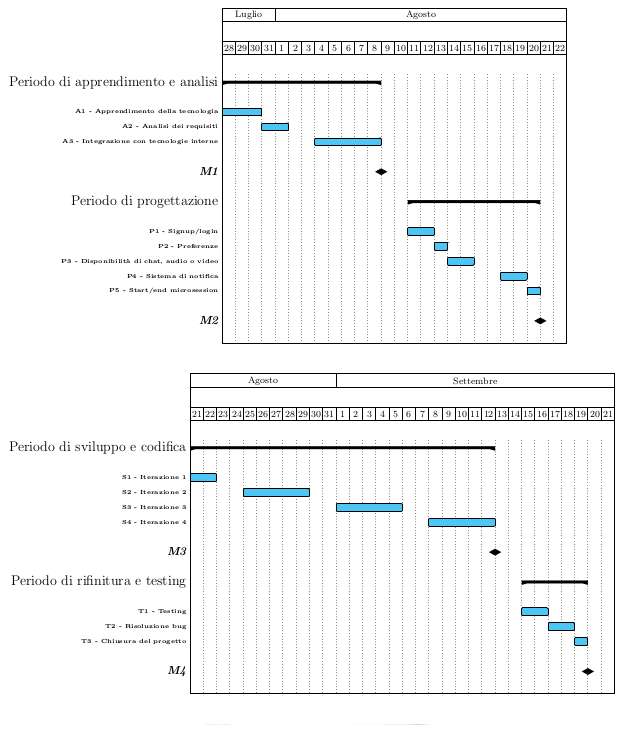
\includegraphics[width=\textwidth]{../immagini/gantt}
\caption{Diagramma di Gantt relativo alla pianificazione del lavoro}  
\end{figure}

